\paragraph{Implementation Tiled Matrix Multiplication}

After a great explanation of how to apply the tiling technique to the matrix multiplication operation, we present the CUDA implementation. As we said, the goal of tiled matrix multiplication with CUDA is to optimize the matrix multiplication process by taking advantage of shared memory (small, fast memory space accessible to all threads within the same block).

\highspace
\begin{flushleft}
    \textcolor{Green3}{\faIcon{book} \textbf{Introduction to the implementation}}
\end{flushleft}
The main core of the implementation is about \textbf{tile indexing}. It can be 1 or 2 dimensional. In the following figures, to understand the logic, we show 2 dimensional indexing, which is more natural.
\begin{itemize}
    \item When each thread loads the input from the original matrix ($M$ or $N$), it needs an index.
    \begin{lstlisting}[language=C++]
int Row = by * blockDim.y + ty;
int Col = bx * blockDim.x + tx;
// 2D indexing for accessing Tile 0:
    M[Row][tx]
    N[ty][Col]\end{lstlisting}
    At each iteration, each thread in a block considers the same row of the matrix $M$ and the same column of the matrix $N$. To distribute the workload among the threads, we assign each thread to each column of the matrix $M$ (using the unique index \texttt{tx}, the index of the thread in the CUDA block), and with the same reasoning, we assign each thread to each row of the matrix $N$. The row in the matrix $M$ is fixed, but the column is taken entirely by the assignment of all threads in the block (using \texttt{tx}).

    In the following figure, we see that the row in the matrix $M$ is fixed, but the column is fully occupied thanks to the assignment of all threads in the block (using tx).
    \begin{figure}[!htp]
        \centering
        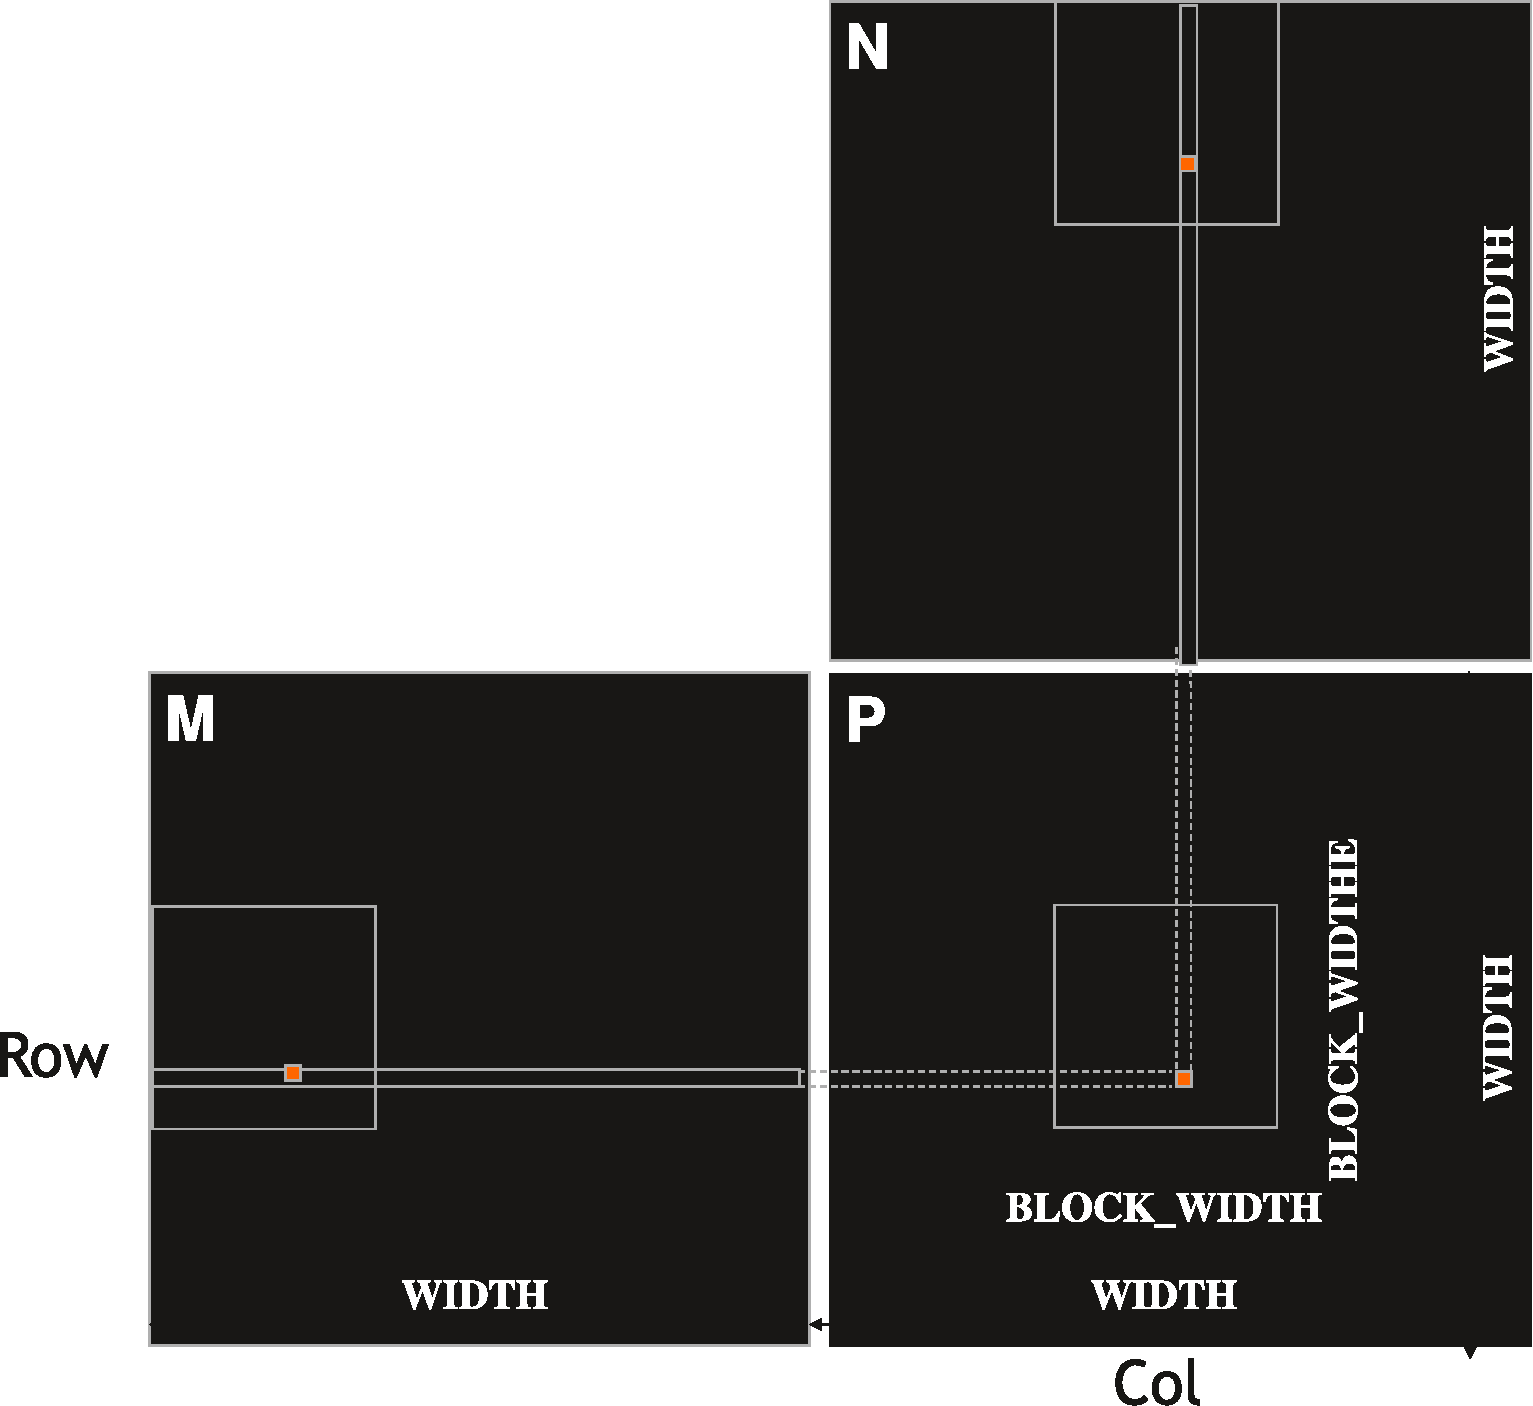
\includegraphics[width=.65\textwidth]{img/cuda-implementation-tile-1.pdf}
    \end{figure}
    \newpage
    When the first phase is finished, we move on to the second tile. For this reason, we use a kind of \textbf{offset} given by the formula $p \times \texttt{TILE\_WIDTH}$ ($\texttt{TILE\_WIDTH} = \texttt{BLOCK\_WIDTH}$), where $p$ is the number of the phase (at the beginning zero, then one, and so on).

    In the following image, we see that at phase 1, to load the tile 1, we use the formula:
    \begin{lstlisting}[language=C++]
// 2D indexing for accessing Tile 1:
M[Row][1 * TILE_WIDTH + tx]
N[1 * TILE_WIDTH + ty][Col]\end{lstlisting}
    \begin{figure}[!htp]
        \centering
        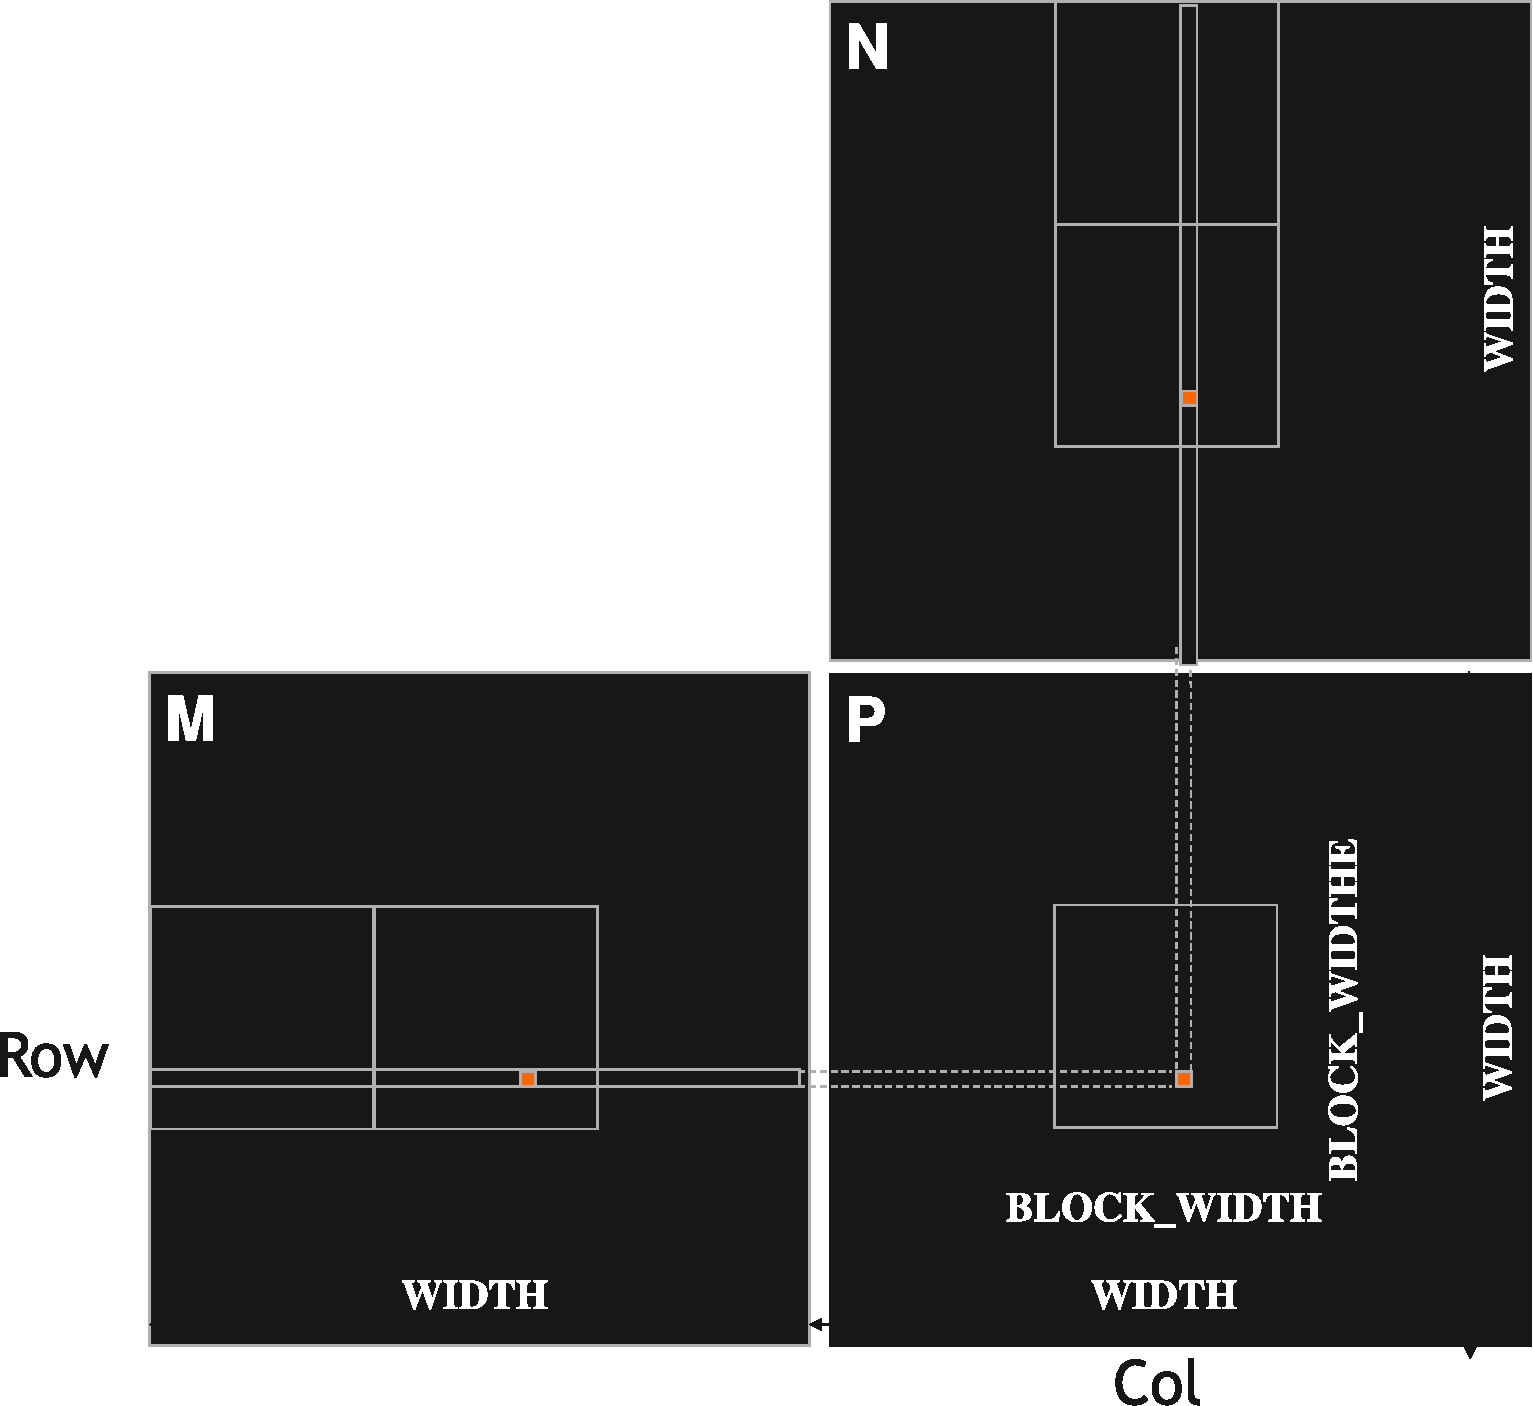
\includegraphics[width=.7\textwidth]{img/cuda-implementation-tile-2.pdf}
    \end{figure}
\end{itemize}

\newpage

\highspace
\begin{flushleft}
    \textcolor{Green3}{\faIcon{tools} \textbf{CUDA code}}
\end{flushleft}
\begin{lstlisting}[language=C++]
#define TILE_WIDTH 16

__global__ void MatrixMulKernel(
    float* M, float* N, float* P, int Width
) {
    __shared__ float ds_M[TILE_WIDTH][TILE_WIDTH];
    __shared__ float ds_N[TILE_WIDTH][TILE_WIDTH];

    int bx = blockIdx.x; int by = blockIdx.y;
    int tx = threadIdx.x; int ty = threadIdx.y;

    int Row = by * blockDim.y + ty;
    int Col = bx * blockDim.x + tx;
    float Pvalue = 0;

    // Loop over the M and N tiles 
    // required to compute the P element
    int bound = Width / TILE_WIDTH;
    for (int p = 0; p < bound; ++p) {
        // Collaborative loading of M and N tiles
        // into shared memory
        ds_M[ty][tx] = M[Row * Width + p * TILE_WIDTH + tx];
        // = M[Row][p * TILE_WIDTH + tx]
        ds_N[ty][tx] = N[(p * TILE_WIDTH + ty) * Width + Col];
        // = N[p * TILE_WIDTH + ty][Col]
        __syncthreads();

        for (int i = 0; i < TILE_WIDTH; ++i) {
            Pvalue += ds_M[ty][i] * ds_N[i][tx];
        }
        __syncthreads();
    }
    P[Row * Width + Col] = Pvalue;
}
\end{lstlisting}
\begin{itemize}
    \item \textbf{Index variables}:
    \begin{itemize}
        \item \texttt{bx} and \texttt{by} are the \textbf{block indices} in the $x$ and $y$ directions.
        \item \texttt{tx} and \texttt{ty} are the \textbf{thread indices} within a block.
        \item \texttt{Row} and \texttt{Col} are the \textbf{row and column indices of the element in the output matrix}.
    \end{itemize}

    \item \textbf{Main Loop}: \texttt{ph} (phase) determines which tile is currently being processed.
    
    \item \textbf{Loading Tiles into Shared Memory}:
    \begin{itemize}
        \item Each thread loads one element from the current tile of $M$ and $N$ into shared memory.
        \item \texttt{ds\_M[ty][tx]} loads an element from $M$.
        \item \texttt{ds\_N[ty][tx]} loads an element from $N$.
        \item \texttt{\_\_syncthreads()} is called to ensure all threads have loaded their elements before proceeding.
    \end{itemize}

    \item \textbf{Matrix Multiplication within a Tile}. Once the tiles are loaded into shared memory, each thread computes the \textbf{partial dot product for the corresponding element} in the output matrix. The nested loop (second for loop) accumulates the product of elements from $M$ and $N$.

    \item Finally, after all tiles have been processed, the \textbf{final value is stored} in the output matrix $P$.
\end{itemize}

\highspace
\begin{flushleft}
    \textcolor{Green3}{\faIcon{check-circle} \textbf{Final consideration}}
\end{flushleft}
A bigger block is better and the reason is simple. \textbf{Bigger tiles mean more threads per block}. For example:
\begin{itemize}
    \item \texttt{TILE\_WIDTH} of 16 results in $16 \times 16 = 256$ threads per block.
    \item \texttt{TILE\_WIDTH} of 32 results in $32 \times 32 = 1024$ threads per block.
\end{itemize}
Therefore, the \emph{workload} per phase is:
\begin{itemize}
    \item \texttt{TILE\_WIDTH} = 16:
    \begin{itemize}
        \item Each block performs 512 ($2 \times 256$) float loads from global memory.
        \item Executes \textbf{8192} ($256 \times \left(2 \times 16\right)$) \textbf{multiply-add operations} (16 floating point operations for each memory load).
    \end{itemize}

    \item \texttt{TILE\_WIDTH} = 32:
    \begin{itemize}
        \item Each block performs 2048 ($2 \times 1024$) float loads from global memory.
        \item Executes \textbf{65536} ($1024 \times (2 \times 32)$) \textbf{multiply-add operations} (32 floating point operations for each memory load).
    \end{itemize}
\end{itemize}
Although a larger block might be better, shared memory is not infinite. It depends on the implementation. If we take a classic Streaming Multiprocessor (SM) with 16KB of shared memory, when we do a memory usage analysis:
\begin{itemize}
    \item \texttt{TILE\_WIDTH} = 16:
    \begin{itemize}
        \item Uses \textbf{2KB} ($2 \times 256 \times 4\text{B}$) \textbf{of shared memory per block}.
        \item Allows up to \textbf{8 blocks per SM} in parallel execution ($8 \times 256$ threads $=$ 2048 threads).
    \end{itemize}
    This allows up to 4096 ($8 \times 512$) pending loads (2 per thread, 256 per block).
    
    \item \texttt{TILE\_WIDTH} = 32:
    \begin{itemize}
        \item Uses \textbf{8KB} ($2 \times 32 \times 32 \times 4\text{B}$) \textbf{of shared memory per block}.
        \item Allows up to \textbf{2 blocks per SM} in parallel execution (limited by thread count). If a GPU limits the thread count to 1536 threads per SM, the number of blocks per SM is reduced to one!
    \end{itemize}
\end{itemize}
Using \texttt{\_\_syncthreads()} ensures that all threads reach a barrier before continuing, which can \textbf{temporarily reduce the number of active threads}. \textbf{More blocks per SM can be beneficial to balance memory usage and thread count}.

\highspace
In summary, \textbf{choosing the right tile size and efficiently managing shared memory and threads are critical to optimizing GPU performance}. This balance affects how many operations can be performed simultaneously and how effectively memory is used.
